\documentclass{article}
\usepackage[T1]{fontenc}
\usepackage{lmodern}
\usepackage{graphicx}
\usepackage{amsmath,amssymb}
\usepackage[a4paper,margin=2cm]{geometry}
\usepackage[absolute,overlay]{textpos}
\setlength{\TPHorizModule}{1mm}
\setlength{\TPVertModule}{1mm}
\usepackage[indonesian]{babel}
\usepackage{hyperref}
\setlength{\emergencystretch}{2em}
% unit: Halaman 44

\begin{document}

% === Halaman 44 (llm) ===

\section*{Kriptanalisis}

\begin{itemize}
    \item \textbf{Kriptanalisis} (\textit{cryptanalysis}): ilmu dan seni untuk memecahkan chiperteks menjadi plainteks tanpa mengetahui \textit{kunci} yang digunakan.
    \item Pelakunya disebut \textbf{kriptanalis}
    \item Kriptanalisis merupakan "lawan" kriptografi
    \item Teknik kriptanalisis sudah ada sejak abad ke-9.
\end{itemize}

\vspace{10mm}

Kriptanalisis dikemukakan pertama kali oleh seorang ilmuwan Arab pada Abad IX bernama \textit{Abu Yusuf Yaqub Ibnu Ishaq Ibnu As-Sabbah Ibnu 'Omran Ibnu Ismail Al-Kindi}, atau yang lebih dikenal sebagai \textbf{Al-Kindi}.

% deskripsi: Gambar prangko yang menampilkan ilustrasi Al-Kindi sedang menulis
% bbox normalisasi: [0.6780, 0.3980, 0.8670, 0.8630]
\begin{textblock*}{39.69mm}(142.38mm,118.21mm)
\noindent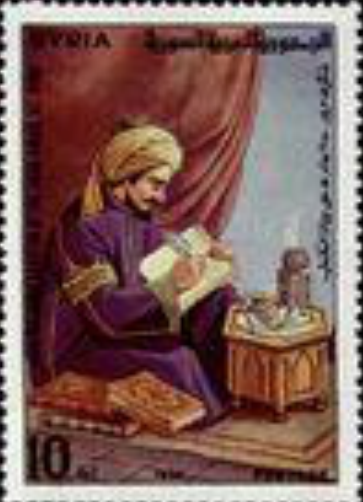
\includegraphics[width=39.69mm,height=138.10mm]{../../images/llm/page_044_img_01.png}%
\end{textblock*}

\end{document}
